\documentclass[a4paper,10pt,english]{article}
%\documentclass[12pt,preprint]{aastex}
\usepackage[utf8]{inputenc}
\usepackage[margin=0.5in]{geometry} % narrow margins
\usepackage{multicol}
% Document formatting
\setlength{\parindent}{0mm}
\setlength{\parskip}{1.5mm}

\usepackage{amsfonts}
\usepackage{graphicx}
\usepackage{float}
\usepackage{cite}
\usepackage{amsmath}
\usepackage{epsfig,floatflt}
\usepackage{hyperref}
\usepackage{listings}
\usepackage[table,xcdraw]{xcolor}
\usepackage{booktabs}
\usepackage{subfig}
\usepackage{algpseudocode}
\usepackage{algorithm}
%\usepackage{amsmath,graphicx,varioref,verbatim,amsfonts,geometry,amssymb,dsfont,blindtext}
\hypersetup{colorlinks=true}
\usepackage{xcolor}
\usepackage{hhline}
\usepackage[export]{adjustbox}
\definecolor{LightGray}{gray}{0.95}
\definecolor{dkgreen}{rgb}{0,0.6,0}
\definecolor{gray}{rgb}{0.5,0.5,0.5}
\definecolor{mauve}{rgb}{0.58,0,0.82}
\definecolor{mygray}{rgb}{0.9,0.9,0.9}
\definecolor{LightGray}{gray}{0.95}
\lstset{frame=tb,
	language=Python,
	aboveskip=3mm,
	belowskip=3mm,
	showstringspaces=false,
	columns=flexible,
	basicstyle={\small\ttfamily},
	numbers=none,
	numberstyle=\tiny\color{gray},
	keywordstyle=\color{blue},
	commentstyle=\color{dkgreen},
	stringstyle=\color{mauve},
	backgroundcolor=\color{mygray},
	breaklines=true,
	postbreak=\mbox{\textcolor{red}{$\hookrightarrow$}\space}
	%breakatwhitespace=true,
	%tabsize=3
}

%\usepackage[english]{babel}
%\usepackage{fancyhdr}
%\usepackage{lastpage}
%
%\pagestyle{fancy}
%\fancyhf{}
%
%\rfoot{Page \thepage \hspace{1pt} of \pageref{LastPage}}
\pagenumbering{arabic}

\begin{document}
\title{FYS-STK4155 Project 2}
\author{Bendik Steinsvåg Dalen \& Gabriel Sigurd Cabrera}
%\maketitle

\maketitle
\begin{abstract}
\end{abstract}

\begin{multicols*}{2}

\section*{Introduction}
\label{sec:introduction}

\section*{Data}
\label{sec:data}

\subsection*{Credit Card Data}

Our first dataset contains real credit card metadata for 30,000 people, in the form of a \texttt{.xls} file; each given datapoint (or person) has 23 features and one \textit{binary output} denoting whether or not they've defaulted on their credit card debt.  These features can be summarized as follows:

\begin{table}[H]
\center
\small
\begin{tabular}{c l l}
Feature No. & Description & Data Type\\
\hline
1 & Total Credit Given & Continuous\\
2 & Gender & Categorical\\
3 & Education & Categorical\\
4 & Marital Status & Categorical\\
5 & Age & Continuous\\
6-11 & Month-Wise Repayment Status & Categorical\\
12-17 & Month-Wise Bill Statement & Continuous\\
18-23 & Month-Wise Amount Paid & Continuous
\end{tabular}
\end{table}

For more detailed information regarding this dataset, and the file itself, visit \url{https://archive.ics.uci.edu/ml/datasets/default+of+credit+card+clients}

\subsection*{The Franke Function}

The second dataset will be given by the \textit{Franke function}, which is defined as follows:

\begin{align*}
f(x,y) &= \frac{3}{4} \exp \left( -\frac{(9x-2)^2}{4} -\frac{(9y-2)^2}{4} \right) \\ &+ \frac{3}{4} \exp \left( -\frac{9x+1}{49} -\frac{9y+1}{10} \right) \\ &+ \frac{1}{2} \exp \left( -\frac{(9x-7)^2}{4} -\frac{(9y-3)^2}{4} \right) \\ &- \frac{1}{5} \exp \left( -(9x-4)^2 - (9y-7)^2 \right)
\end{align*}

We will be solving the Franke function for 100 $x$-values and 100 $y$-values in the range $[0,1]$, leaving us with a grid containing a total of 10000 $xy$ coordinate pairs.  This leaves us with the values plotted in Figure \ref{fig_Franke}.

\begin{figure}[H]
	\centering
	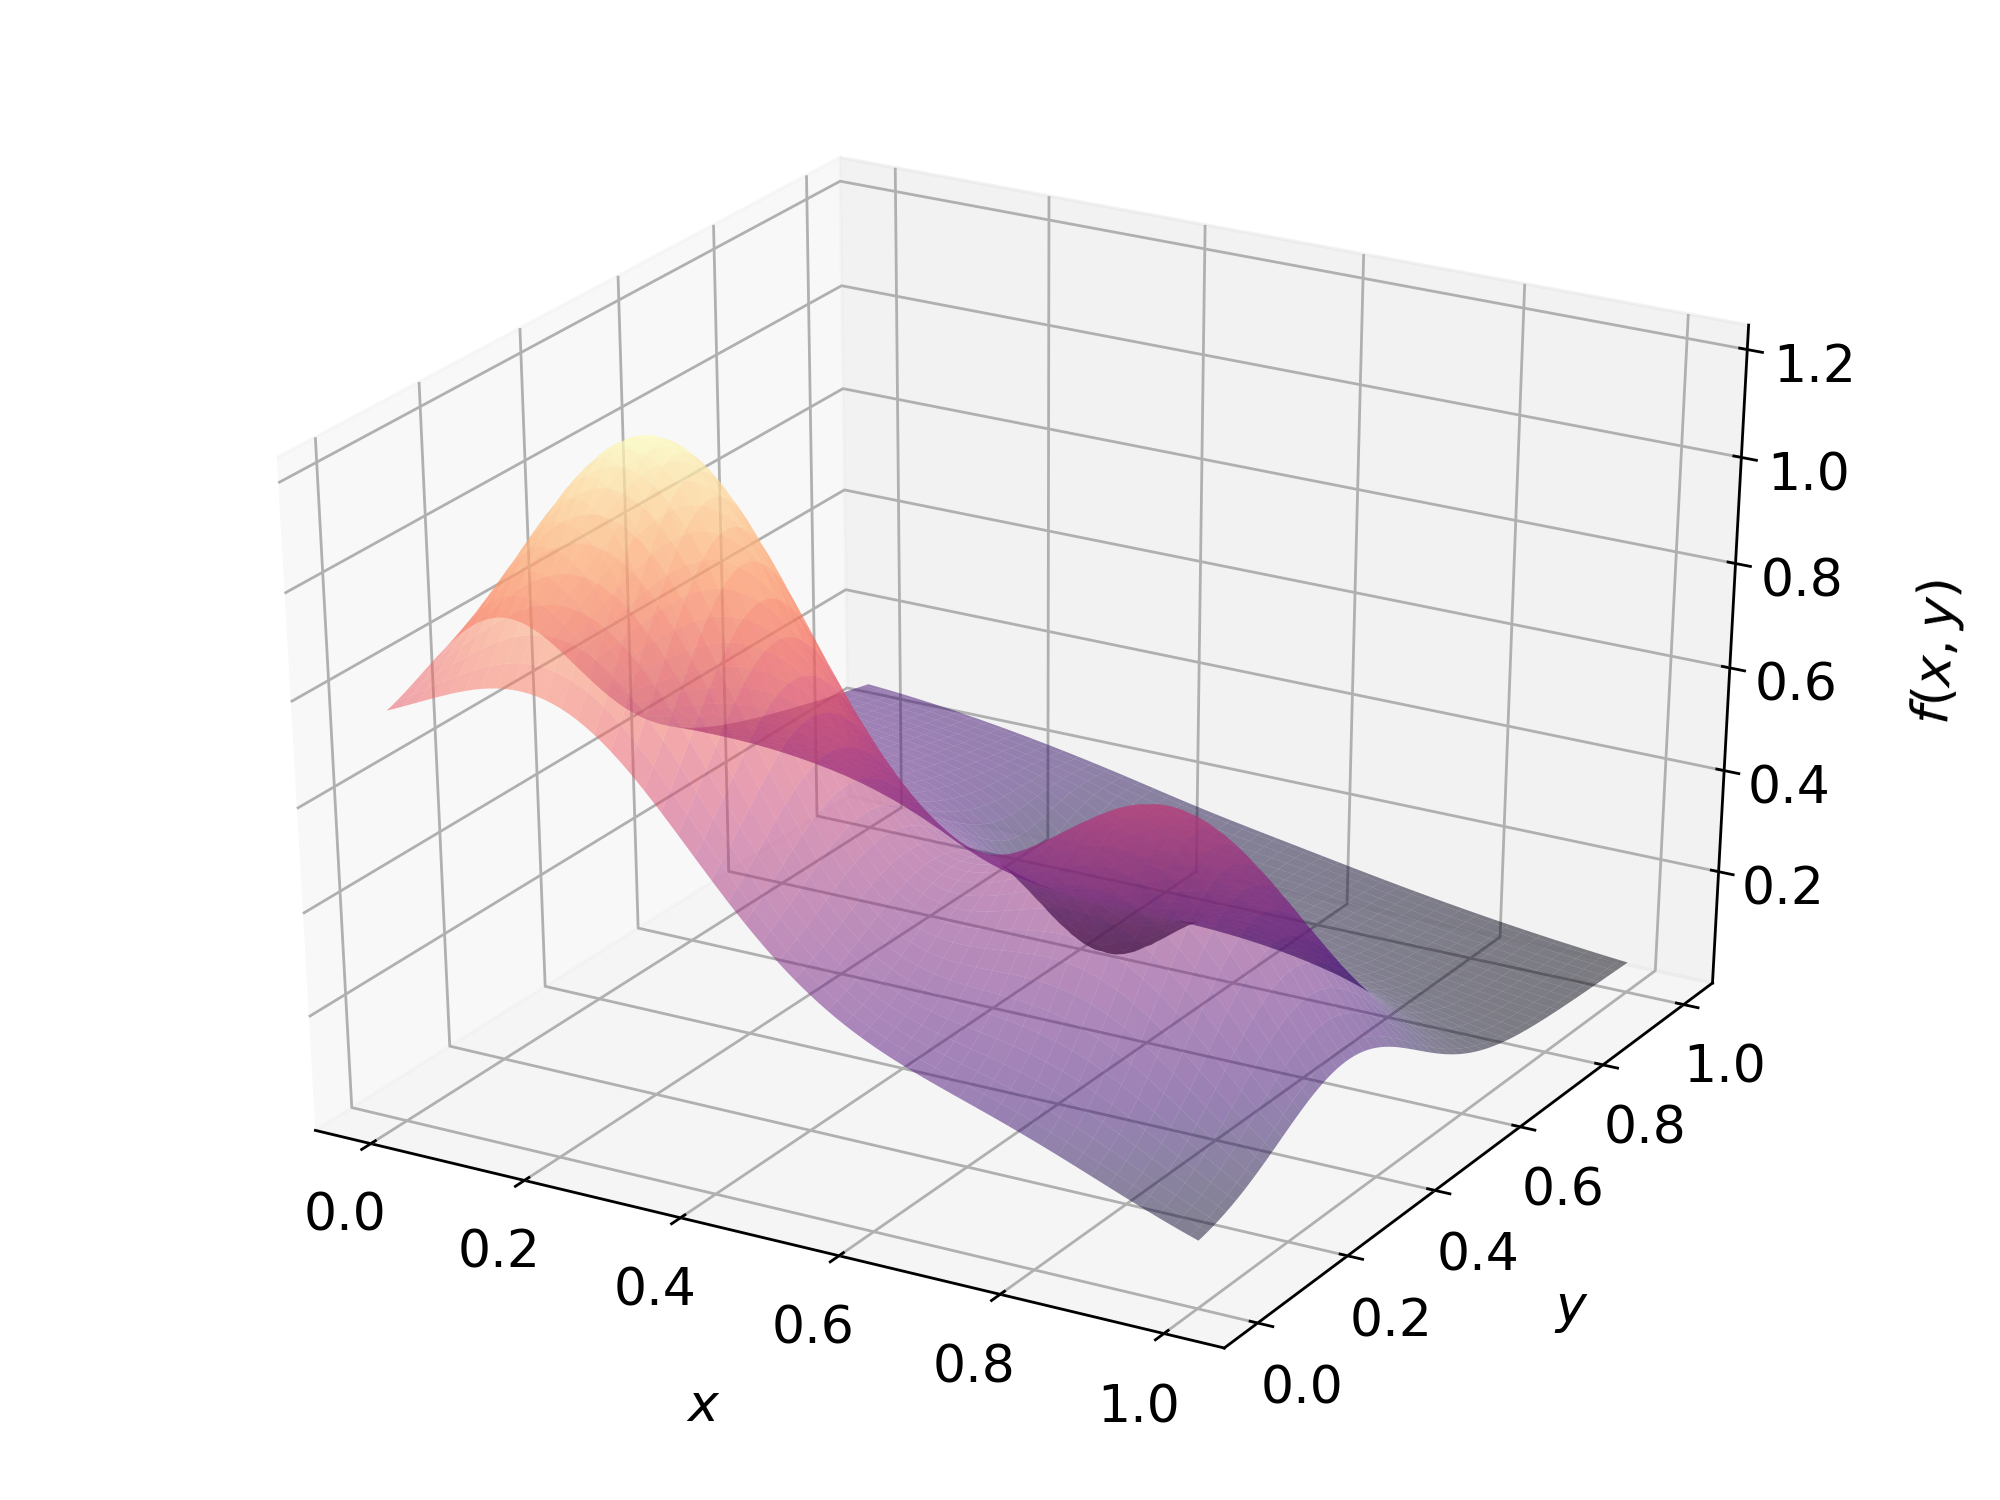
\includegraphics[width = 0.5\textwidth, center]{Franke.png}
	\caption{The \textit{Franke function} for $x$ and $y$ values ranging from zero to one. \label{fig_Franke}}
\end{figure}

In addition, we will also be adding \textit{Gaussian noise} to each value $f(x,y)$, such that we are left with values as seen in Figure \ref{fig_Franke_noise}.

\begin{figure}[H]
	\centering
	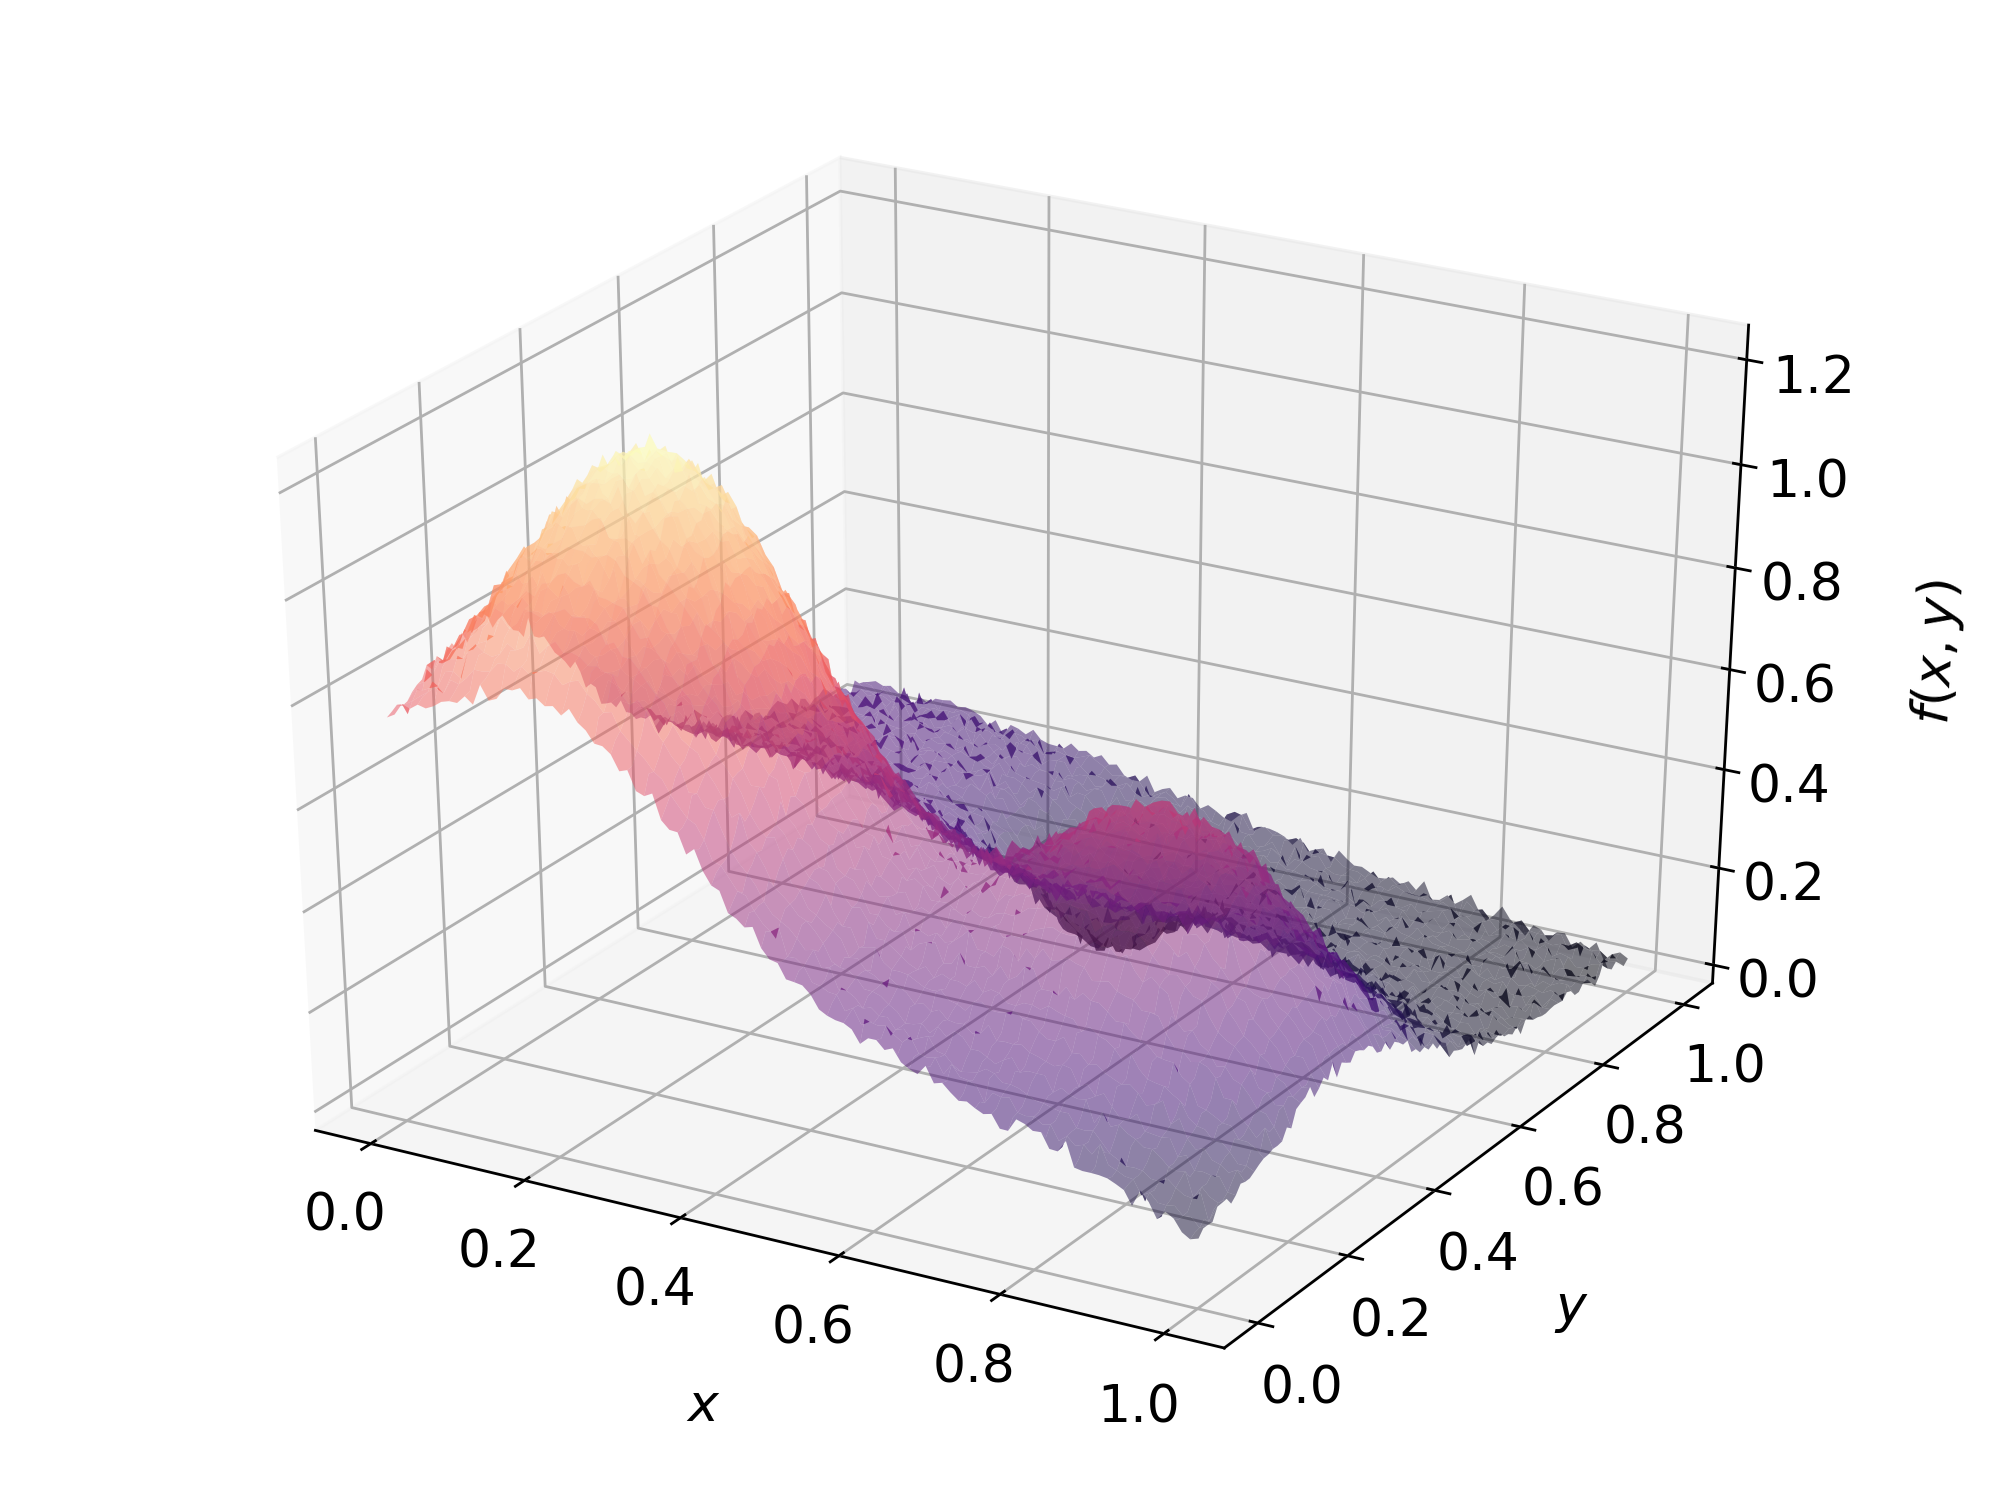
\includegraphics[width = 0.5\textwidth, center]{Franke_noise.png}
	\caption{The \textit{Franke function} for $x$ and $y$ values ranging from zero to one, with a Gaussian noise $N(0,0.01)$\label{fig_Franke_noise}}
\end{figure}

\section*{Method}

\subsection*{Logistic Regression}

The first technique we will be using is called \textit{logistic regression} – we will be using the \textit{sigmoid function} as our \textit{activation function}\footnote{A function that restricts the \textit{range} of predicted outputs.}:

\begin{equation}
\label{eq_sigmoid}
\sigma(x) = \frac{1}{1 + e^{-x}}
\end{equation}

We will also need its derivative:

\begin{equation}
\label{eq_diff_sigmoid}
\sigma^\prime(x) = \sigma(x) (1 - \sigma(x))
\end{equation}

Logistic regression is an iterative two-part process consisting of repeated \textit{feed-forward} and \textit{backpropagation} loops between an \textit{input layer} and \textit{output layer}.  Assume that we have an input matrix $\mathbf{X} \in \mathbb{R}^{p \times n}$ and output matrix $\mathbf{y} \in \mathbb{R}^{q \times n}$, where $n$ is the number of \textit{datapoints}, $p$ is the number of \textit{features}, and $q$ is the number of \textit{labels}.  Knowing this, we can generate a matrix of weights $\mathbf{W} \in \mathbb{R}^{q \times p}$ and vector of biases $\mathbf{b} \in \mathbb{R}^q$ such that:

\begin{equation*}
w_{ij} = N(0, 0.5); \qquad b_i = N(0, 0.5)
\end{equation*}

Where $N(\text{mean}, \text{std})$ is the \textit{normal distribution}.  To implement the feed-forward portion of the algorithm, we use matrix multiplication to predict an output $\hat{\mathbf{y}}$ with the given weights:

\begin{equation*}
\hat{\mathbf{y}} = \sigma( \mathbf{w} \mathbf{X} + \mathbf{b} )
\end{equation*}

For simplicity, we will define $\mathbf{z} \equiv \mathbf{w} \mathbf{X} + \mathbf{b}$.

Next, we want to optimize our weights via backpropagation, which requires the use of gradient descent.  Specifically, we want to find $dw_{ij} = \frac{\partial C}{\partial w_{ij}}$, where $C$ is a \textit{cost function}, and $w_{ij} - dw_{ij}$ reduces $C$; to find such a value, we use the multivariable \textit{chain rule} to rewrite $dw_{ij}$:

\begin{equation*}
dw_{ij} = \frac{\partial C}{\partial w_{ij}} = \frac{\partial C}{\partial \hat{y}_i} \frac{\partial \hat{y}_i}{\partial z_i} \frac{\partial z_i}{\partial w_{ij}} = \delta_i \frac{\partial z_i}{\partial w_{ij}}
\end{equation*}

The intent of repeating this process is to reduce our cost function until a local or global minimum is reached and an optimal set of $\mathbf{W}$ and $\mathbf{b}$ are computed.  If we use the \textit{mean squared error} as our cost function, this can be rewritten in matrix form as follows:

\begin{equation}
\label{eq_backprop_output}
d\mathbf{w} = [2(\hat{\mathbf{y}} - \mathbf{y}) \odot \sigma^\prime(\hat{\mathbf{y}})] \otimes \mathbf{X}
\end{equation}

One full feedforward–backpropagation iteration is known as a \textit{batch}; if $N$ datapoints are calculated in a single batch, we say that the \textit{batch size} is $N$, and $d\mathbf{w}$ is averaged over each input.

Once a batch is complete, the updated weights and biases are used in the next batch, and so on for each subsequent batch. When all the batches have been evaluated, we say that an \textit{epoch} has been completed; many epochs are often required to properly optimize a set of weights and biases.

\subsection*{Neural Networks}

The second technique we will explore is the usage of \textit{multi-layer neural networks}; as with logistic regression, there exists an input layer and output layer and a set of weights and biases.  Now, however, we also have a variable number of \textit{hidden layers} $L-1$, each consisting of a variable number of \textit{nodes}.

As with logistic regression, we must randomly initialize a set of weights – this time, however, we will need several weight matrices and bias vectors; specifically, we need an amount equal to the number of hidden layers, plus one.  Each weight matrix $w^\ell$ must have as many rows as there are nodes in the subsequent layer, and as many columns as there are in the preceeding layer; each bias vector must be as large as the subsequent layer.

The feed-forward portion of the algorithm is unchanged, with the exception that the process must be repeated layer-by-layer, for each set of weights accompanying the product in question; the backpropagation, however, is more complex.

To update all of our weights, we begin by using (\ref{eq_backprop_output}) on the \textit{last} set of weights\footnote{Those between the final hidden layer and output layer.} $\mathbf{w}^\textsc{l}$.  Once this has been accomplished, we can update these weights and use the following equation to find the remaining $d\mathbf{w}^\ell$:

\begin{equation*}
d\mathbf{w}^\ell = (\mathbf{W}^{\ell+1})^\textsc{t} \delta^{\ell+1}_i \odot \sigma^\prime(\mathbf{z}^\ell)
\end{equation*}

\subsection*{Mean Squared Error}

To get a measure of success with respect to the implemented method and parameters, we can calculate the mean difference in the squares of each measured output $y_i$ and their respective predicted outputs $\hat{y}_i$:

\begin{equation*}
MSE(\mathbf{y}, \mathbf{\hat{y}}) = \frac{1}{N} \sum_{i=1}^{N} (y_i - \hat{y}_i)^2 = \mathbb{E}\left[(\mathbf{y}-\hat{\mathbf{y}})^{2}\right]
\end{equation*}

The lower the $MSE$, the closer the polynomial approximation is to the original dataset.  If it is too low, however, we run the risk of overfitting our dataset, which is not desireable either – fortunately, this not an issue within the scope of this report.

\subsection*{R\textsuperscript{2} Score}

Another measure of success is the \textit{coefficient of determination}, colloquially known as the $R^2$ score, is given by the following expression:

\begin{equation*}
R^2 = 1 - \frac{\sum_{i=1}^N (y_i - \hat{y}_i)^2 }{\sum_{i=1}^N (y_i - \bar{y}_i)^2 }
\end{equation*}

The closer $R^2$ is to one, the closer the polynomial approximation is to the input/output dataset, although a perfect score can once again arise due to overfitting just as in the case of the $MSE$.

\subsection*{ROC}

The \textit{ROC} (short for \textit{receiver operating characteristic}) of a binary classifier is a measure of how well a model performs, by accumulating and comparing the rate of true positives\footnote{How often \texttt{1} is predicted when \texttt{1} is expected.} (\textit{TPR})
 and rate of false positives\footnote{How often \texttt{1} is predicted when \texttt{0} is expected.} (\textit{FPR}). These can be calculated as follows:

\begin{equation}
\label{eq_ROC}
TPR = \frac{TP}{TP + FN}; \qquad FPR = \frac{FP}{FP + TN}
\end{equation}

Where $TP$, $FN$, $FP$, and $TN$ are the total number of \textit{true positives}, \textit{false negatives}, \textit{false positives}, and \textit{true negatives}, respectively.

Note that the equations in (\ref{eq_ROC}) are \textit{scalar values} – to construct our curve, we must therefore calculate $TPR$ and $FPR$ for \textit{every datapoint}. Once this is accomplished, the values are ordered such that predicted outputs furthest from $0.5$ are prioritized.  Next, the values are cumulatively summed up and the resulting series are normalized to $1$: normalization is important, since we are interested in \textit{rates} of prediction.

\subsection*{AUC}

The \textit{AUC} (or \textit{area under ROC}) is a measure of model performance; an AUC closer to $1$ suggests that a model is good at correctly making predictions, while an AUC closer to $0$ implies that a model is bad at binary classification.  The AUC of a model is calculated by finding the \textit{area} under the ROC curve of the given model; since the ROC is assumed to be normalized in the range $0$ to $1$, so will the AUC.

\begin{figure}[H]
	\centering
	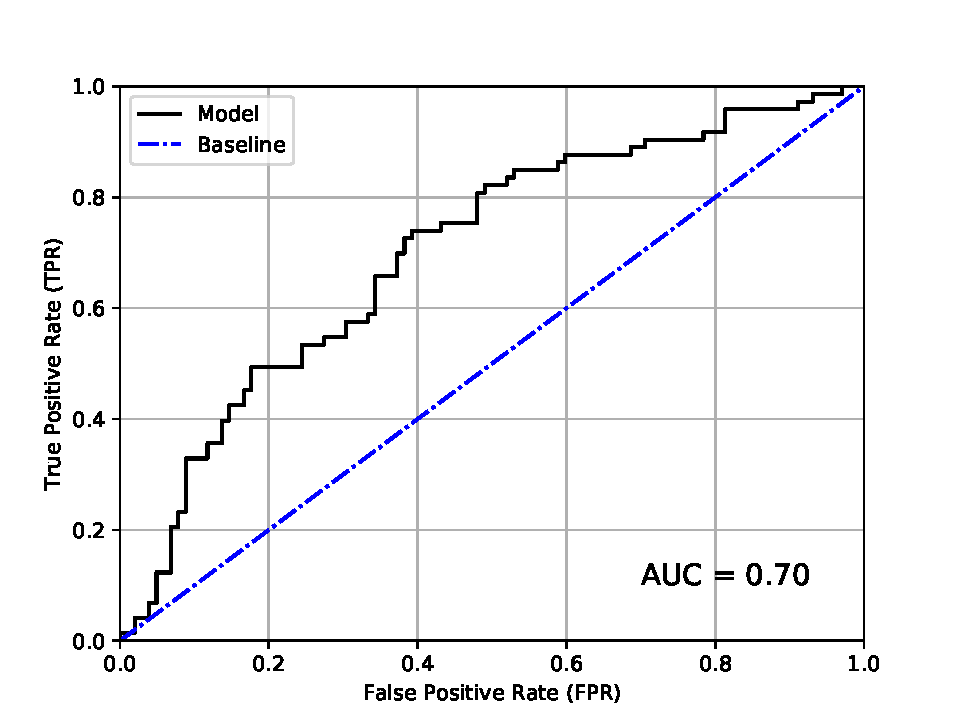
\includegraphics[width = 0.5\textwidth, center]{roc_sample.pdf}
	\caption{An example $ROC$ curve with its $AUC$.\label{fig_roc_sample}}
\end{figure}

\section*{Results}

\section*{Discussion}

\section*{Conclusion}

\bibliography{bib}{}
\bibliographystyle{ieeetr}
\end{multicols*}{2}
\end{document}